\chapter{Implementation}

\section{Framework}

\emph{Status: Not Started}

\begin{itemize}
\item Entirely based on Python
\item Explain dropping of Nodejs in favor of Python (due to Celery)
\end{itemize}

\subsection{API}

\emph{Status: Not Started}

\begin{itemize}
\item POST, DELETE and GET methods
\end{itemize}

\subsection{Task Queue \& Celery}

\emph{Status: Not Started}

\begin{itemize}
\item Celery for Task Queue
\item Flower utility app
\item Based RabbitMQ
\end{itemize}

\subsection{Configuration}

\emph{Status: Not Started}

\begin{itemize}
\item Config.xml
\item XSD schema
\end{itemize}

\subsection{Engine Adapters}

\emph{Status: Not Started}

\begin{itemize}
\item Thin clients for engines
\item Hybrid
\end{itemize}

\emph{Status: Not Started}

\begin{itemize}
\item Functional testing and unit testing
\end{itemize}

\section{Engines}

\subsection{Collaborative Recommender: In Common}

\emph{Status: Not Started}

\begin{itemize}
\item Collaborative filtering
\item Real-time
\item Data and domain agnostic
\item Based on Go
\item API
\item Based on graphical databases and nodes
\item Figure to show diagram for adding, deleting and reading
\item Unit testing
\end{itemize}

\subsection{Content-Based Recommender: Item Similarity}

\emph{Status: Not Started}

\begin{itemize}
\item Content-based filtering
\item Silex, MongoDB, Doctrine ODM
\item Requires master data
\item Show diagram for adding, deleting and reading
\item How similarity is calculated
\item Unit testing
\end{itemize}

\subsection{Hybrid Recommender: Weighted}

\emph{Status: Not Started}

\begin{itemize}
\item Weight
\item No specific implementation, assisting methods to access components, rest job of the adapter
\end{itemize}

\section{Demo Domain System: Magento}

Section \ref{architecture-domain-systems} discussed the definition and characteristics of \emph{domain systems} as systems founded on extensive domain knowledge. Although the focus of the project is on the framework and recommendation engines, it was clear from the beginning that they needed to be trialed and demonstrated on a complex domain system. Since e-commerce websites are amongst the major users of recommender systems, demonstrating the work on an e-commerce system. As proposed, the e-commerce software \emph{Magento} has been used for this. \citet{aheadworks14} analysed \emph{Alexa}'s 1 million top sites index and found that Magento was the leading open-source e-commerce software with a market share of 30 percent in 2014.

\begin{figure}[!ht]
    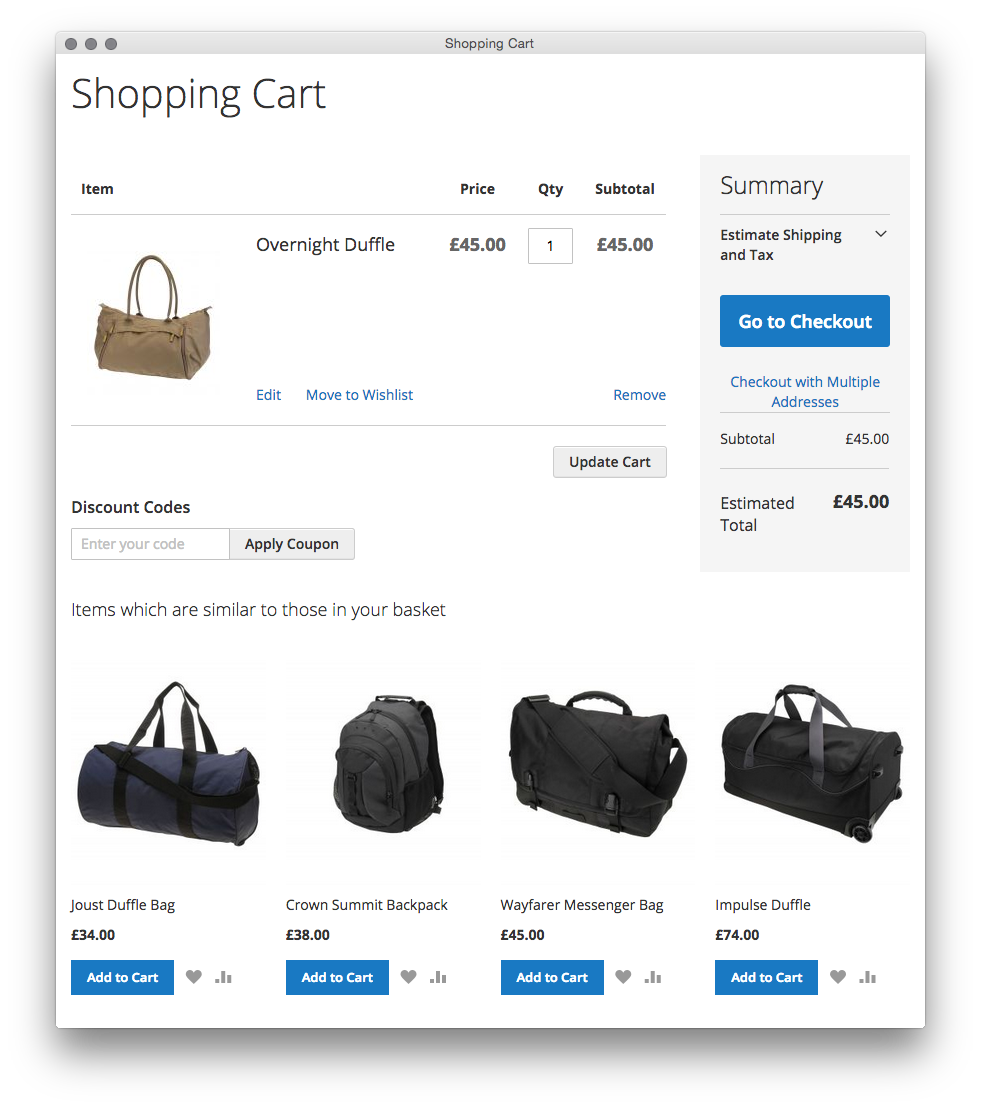
\includegraphics[width=\textwidth,center]{screens/basket.png}
    \caption{Content-based recommendations on shopping basket}
    \label{fig:implementation-magento-basket}
\end{figure}

The authors of Magento are working on a full rewrite of their platform called Magento2 to be released late 2015. This project uses the first release candidate published in March 2015. Albeit Magento2 comes with fundamental technical changes, they do not necessarily make a difference to the purposes of demonstration. Nonetheless the support of the dependency manager \emph{Composer} was principally important to distinct between custom and core code. Secondly, the sample data generator was useful to demo with realistic data.

\subsection{Events}
\label{implementation-magento-events}

Magento comes with an event subsystem in which observers can subscribe to various events -- from very low-level to very specific functions. This helped to keep the required code clean and short.

The following cases are recorded and posted to the framework as events:

\begin{itemize}
\item \emph{Customer views a product}
\item \emph{Customer adds or removes a product to their wishlist}
\item \emph{Customer adds a product to their basket}
\end{itemize}

There are more cases which are interesting in an e-commerce context such as the actual purchase of items. The aforementioned cases have been symbolicly chosen as they do not require too many steps to reproduce. In contrary, a checkout on Magento is a longer process which requires documentation and can be time-consuming on slow development environments. Above all, the \emph{In-Common} recommender requires three occurances of a case to produce a recommendation: the first customer performing a behaviour with another customer doing the same as well as one which the first customer has not experienced yet.

Finally, the customer identification is most of the times part of the event data. A customer who has not logged in yet gets a \emph{visitor ID} assigned to by Magento. This allows behavioural analysis and production of recommendations even for logged out users. Once they log in, the \emph{customer ID} can be used so that the recommendations can source from historic sessions. In order to troubleshoot any issues, all requests and responses to the event API of the framework are logged in a file.

\subsection{Master Data}

The master data is exceptionally important for content-based recommenders as they source their recommendations from similarities between item features. In the Magento context, master data refers to the product catalogue and is sent to the framework as regular events. Again, the event subsystem allows to observer product catalogue changes and notify the framework in real-time. On first run or if explicitly wished, the catalogue data can be exported as a whole with a command-line script. This is known as full export and the data is transmitted in batches.

Magento implements an \emph{entity-attribute-value (EAV)} model. \emph{Entities} are a type of product such as books and phones and are called \emph{attribute sets} in Magento. \emph{Attributes} are fields within a product catalogue and have a value type such as text or numeric amounts. The \emph{values} can be entered freely or chosen from an editable list. The EAV model basically describes that although the number of attributes in a catalogue is vast, only a subset of those are relevant and applicable to an entity -- in practice it means that the attribute \emph{number of pages} is relevant for a book but not for a phone.

\begin{figure}[h]
    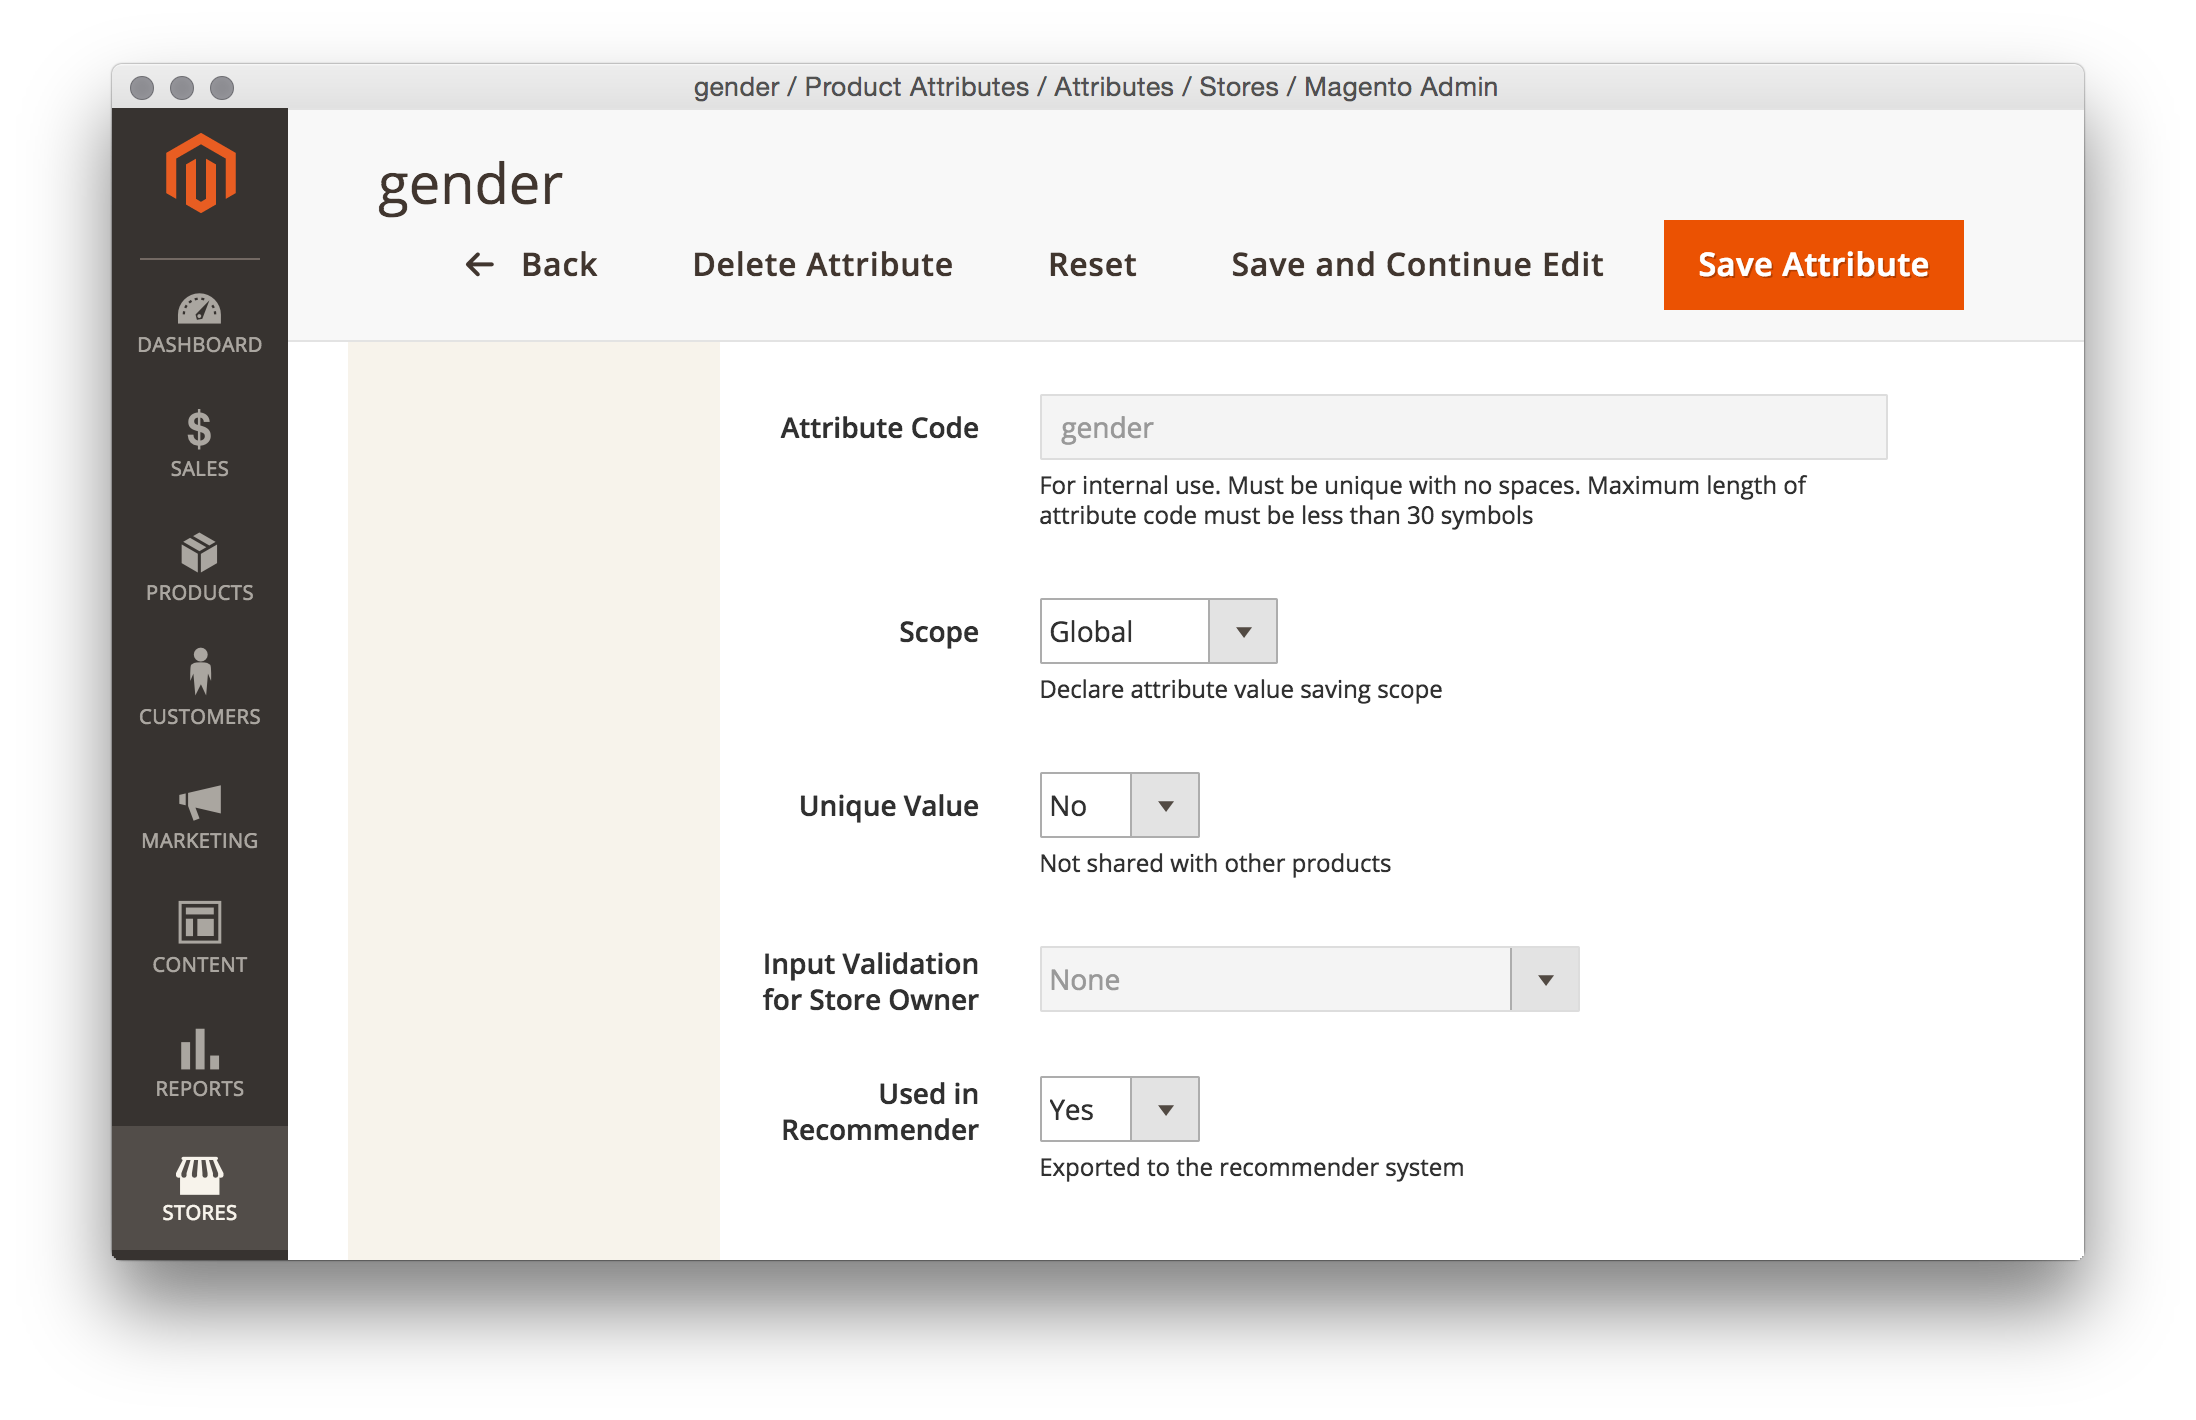
\includegraphics[width=\textwidth,center]{screens/masterdata.png}
    \caption{Manage Master Data in the Back Office of Magento}
    \label{fig:implementation-magento-master-data}
\end{figure}

Magento provides a user interface in the back office to manage these attributes and attribute sets; thus means that the master data can vary extensively between Magento instances. There are so called \emph{system attributes} which remain the same on any Magento instance but the majority of the relevant data would be merchant-specific. In accomodate this, the demo project implements a way for the merchant to mark attributes as \emph{Used in Recommender} which are to be exported to the framework, as shown in figure \ref{fig:implementation-magento-master-data}. However, as the demo project relies on the samle data generator of Magento which creates attributes, setting that mark had to happen dynamically. The sample data generator and its static source data known as \emph{fixtures} have been extended so that a fixture can be replaced by a customised version.

\subsection{Recommendations}

The integration of recommendations has been implemented in three parts:

First, a thin \emph{client} has been written which performs the request and processes the responses to the recommendation API of the framework. All requests and responses are logged in a file for troubleshooting.

Second, a \emph{recommendation model} is implemented for each recommendation configured in the framework such as \emph{viewed products} and \emph{similar items in basket}. The purpose of these model classes is to provide the IDs the recommendation should be based on -- e.g. current user ID for the \emph{viewed products} and product IDs in the basket for \emph{similar items in the basket}. This is based on the requirement that each recommendation is in relation to something. They do not know internals of how the recommendations work. They are derived from an abstract class which reduces the code size of the individual model classes to a minimum. They return a product collection filtered by the product IDs from the recommendation response.

Third, a \emph{recommendation widget} is provided which handles the display of recommendations to the user. Magento widgets are re-usable, configurable blocks which can be placed on the website. The demo project makes use of a universal product listing widget and feeds it with the product collection provided by the recommendation class. Magento enables developers and merchants to customise the layout of their website in a flexible way. The demo project was able to place these widgets on existing page by supplying short XML files. An exception is the widget on the homepage (seen in figure \ref{fig:implementation-magento-homepage}) as that page is managed by the \emph{content management (sub)system (CMS)} of Magento. Since the homepage is part of the sample data, a customised fixture has been provided, as discussed in the previous section.

\begin{figure}[!ht]
    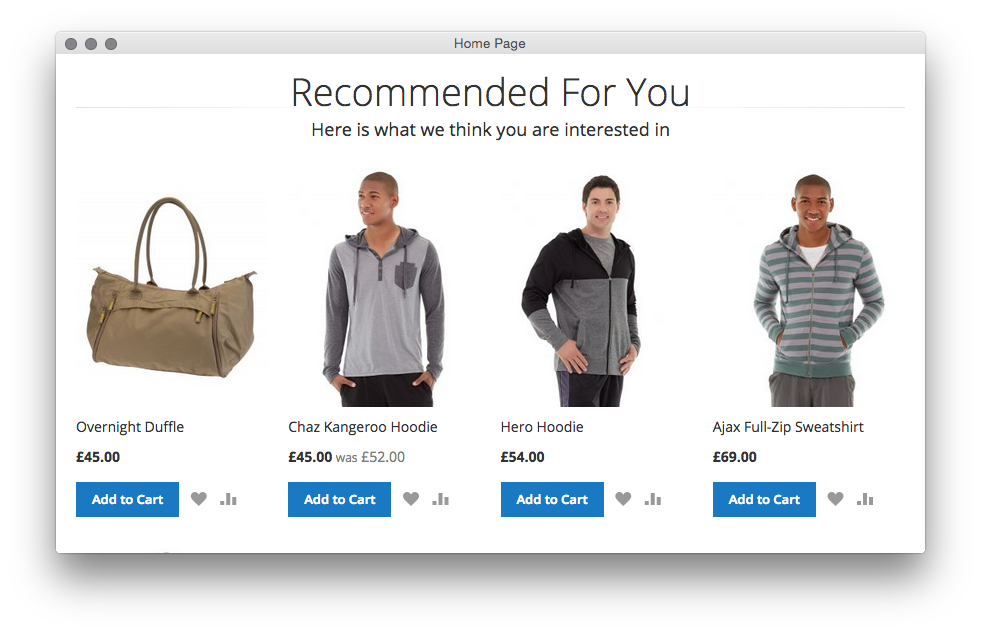
\includegraphics[width=\textwidth,center]{screens/homepage.png}
    \caption{Recommendations on the homepage}
    \label{fig:implementation-magento-homepage}
\end{figure}

\section{Provisioning}

Provisioning refers to the process of preparing an environment which fulfills the requirements to run systems and applications. It involves the installation of languages and libraries as well as proper configuration.

This project relies on the \emph{Linux} operating system and comes with provisioning instructions which are outlined in the next sections.

\subsection{Virtualisation with Vagrant}

\emph{Vagrant} is a software that manages virtual environments -- emulated computer systems also known as \emph{virtual machines} -- for development purposes. It enables a development team to standardise their development environments. This is in particular useful when the computer systems of developers vary from the computer system of the development environment -- e.g. a developer on \emph{Windows} working on a software running on Linux -- or among each other -- i.e. developers using different computer systems which would require provisioning instructions for all computer systems used. In order to run Vagrant, a single configuration file called \emph{Vagrantfile} written in \emph{Ruby} is added to the project's \emph{version control system} such as \emph{Git} and therefore shared with the team.

Vagrant does not do the virtualisation itself but relies on established virtualisation software such as \emph{VirtualBox} and \emph{VMWare}. It also relies on so called \emph{boxes} -- a barebone installation of a computer system minimally configured for Vagrant -- to bootstrap the virtual machine. Although the project works on any Linux distribution, due to the box requirement of Vagrant the Linux distribution \emph{Ubuntu} (version 14.04) has been used.

Another challenge was the fact that the provisioning instruction calling the sample data generation of \emph{Magento} took so long to an extent that it was unbearable for the project demonstration. It was then decided to package a fully provisioned version of the development environment to a ready-to-go box. \emph{HashiCorp} -- the authors of Vagrant -- provide a service called \emph{Atlas} which allows such boxes to be uploaded and available publicly. Boxes for VirtualBox and VMWare have been uploaded to Atlas since Vagrant boxes are specific to the virtualisation software used. It is rather important to notice that VMWare as well as its Vagrant provider -- the middleware between Vagrant and VMWare -- are both commercial whereas VirtualBox is open-source and free.

Vagrant also provides native support for configuration management software as discussed in the next section.

\subsection{Configuration Management with Puppet}

\emph{Puppet} is an open-source software which manages the configuration of \emph{Microsoft Windows}, Linux and other \emph{Unix}-like systems such as \emph{Mac OS X}. This is achieved by describing the expected system configuration in so called \emph{manifest} files written in a custom declarative language derived from \emph{Ruby}. Upon execution, Puppet interprets these manifests into a configuration catalog and compares it against the configuration of one or more new or existing systems. Differences noticed during that step are corrected by Puppet. This ensures the expected configuration on those systems and can be called repetitively.

Puppet supports writing manifests for more than one target environment. In fact, most companies are using Puppet to ensure the same configuration (with some variables) on multiple environments such as production, staging and development. In the Vagrant context the Puppet provisioning is called by default when a new virtual machine is created. However, it can also be called explicitly. Since this project utilises Puppet to provision a development environment only, the manifests are not ready for production. Ensuring that essential security measures amongst others changing default passwords were go beyond the scope of this project.

Manifests can be grouped into so called Puppet \emph{modules}. \emph{PuppetLabs} -- the authors of Puppet - operate a community called \emph{PuppetForge} where modules are shared. This project utilised \emph{PuppetForge} modules e.g. for \emph{Apache} and \emph{PHP} where possible. In reality, most such modules are officially authored by PuppetLabs. Nonetheless, not all modules covered all the configuration needs of this project and were thus custom written inter alia for \emph{Magento}, \emph{Neo4j} as well as the \emph{framework} and \emph{recommendation engines}. The Magento module builds dependencies, creates an Apache virtual host and a MySQL database and runs the Magento installer. The Neo4j module installs and configures the Neo4j server. The recommender module configures both framework and two recommendation engines. It creates Apache virtual hosts, installs dependencies, creates \emph{supervisord} programs to manage background processes and sets up \emph{Celery} and \emph{Flower}. External modules are integrated as Git \emph{submodules}. The provisioning source code in \ref{appendix-soure-code-provisioning} only lists manifests written by the project author.

Puppet can be understood as part of the \emph{infrastructure as code} or \emph{programmable infrastructure} initiatives in organisations. It enables version controlling and automation of provisioning infrastructure. Especially infrastructure based on \emph{cloud computing} and \emph{platform as a service (PaaS)} which involve many but constantly changing (e.g. auto-scaling) systems benefit from this. Alternatives to Puppet are \emph{Chef}, \emph{SaltStack} and \emph{Ansible}.

\subsection{Dependency Management}

Dependency management supports the declaration and installation of libraries a software depends on. Whereas system package managers like \emph{Yum} and \emph{Apt} provide a system-wide solution for packages, dependency managers support versioned solution on a per-project basis. Latter is important as two pieces of software may depend on different versions of a dependency. Furthermore, dependency managers are usually tailored for a programming language and allow the distribution of libraries which may not be available as a Yum or Apt package.

As mentioned in the abstract, this work relies on many open-source projects. It was since particularly important to separate own work from those third-party projects. For this, dependency managers were very essential. The \emph{framework} relies on the Python dependency manager \emph{pip}. The \emph{item-similarity} engine as well as the demo application \emph{Magento} use the PHP dependency manager \emph{Composer}. Finally, the \emph{in-common} engine utilises \emph{gom} which adds per-project capabilities to the overall self-sufficient \emph{Go} dependency manager.